\documentclass{crypto-exercise}
\usepackage{amsthm}
\author[Fiat-Shamir]{Sven Laur}
\contributor{Sven Laur}
\editor{Sven Laur}
\tags{statistical indistinguishability, distributions, zero-knowledge, rejection-sampling, Fiat-Shamir identification scheme}

\renewcommand{\ADVIND}[2]{\ADV^{\mathsf{ind}}_{#1}(#2)}
\newcommand{\REWRITE}{\qquad\scalebox{1.5}{$\rightsquigarrow$}\qquad}
\begin{document}


\begin{exercise}{Standard simulator for the Fiat-Shamir protocol}
Let $\SSS(\beta)$ be the canonical simulator for the Fiat-Shamir sigma protocol, which takes in the challenge $\beta$ and outputs $\alpha, \gamma$ such that for uniformly chosen $\beta\getsu\set{0,1}$ the distribution of $(\alpha,\beta,\gamma)$ coincides with the message distribution between honest prover and verifier. Show that the following simulator construction
\begin{align*}
\begin{fblock}{\VVV_\circ(\phi)}
 &\beta_\circ\getsu\set{0,1}\\
 &(\alpha,\gamma)\gets\SSS(\beta_\circ)\\
 &\beta\gets\VVV_*(\phi,\alpha)\\
 &\IF \beta\neq \beta_\circ\ \THEN \RETURN \bot\\
 &\ELSE \RETURN \VVV_*(\gamma) 
\end{fblock}
\end{align*}   
creates an output distribution $\psi_\circ$ that is statistically $\frac{1}{2}$-distant from the output distribution of malicious verifier $\VVV_*$ that interacts with the honest prover.

\end{exercise}
\begin{solution}
There are many ways how to prove this seemingly evident fact. In this treatment we consider two most revealing approaches.

\vspace*{2ex}
\noindent
\textsc{Proof based on event trees.} The simplest way to visualise what happens in the simulation is to draw the event trees for  the real protocol execution and for the simulation and compare them. For clarity, let us first consider adversaries $\VVV_*$ that do not abort in the real protocol run, i.e., do not output $\bot$. Also, let $k$ be the number of all possible commitment messages $\alpha$. In the Fiat-Shamir protocol, $k=\frac{\phi_e(N)}{4}$ where $\phi_e(\cdot)$ in this context is Euler's totient function. The latter follows from the fact that $\alpha$ is a quadratic residue.   

\begin{figure}[h]
   \centering
   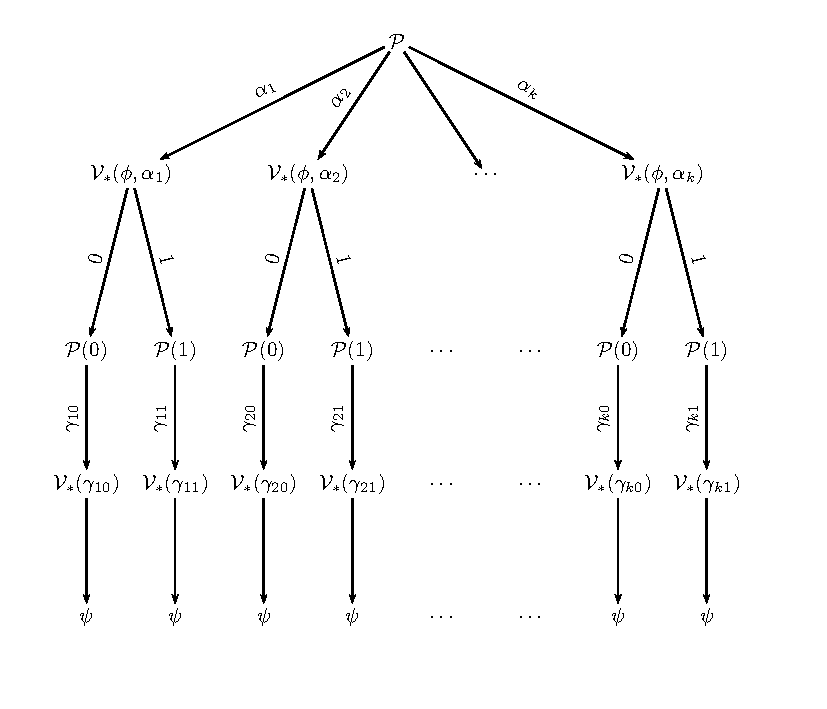
\includegraphics[scale=0.55]{figures/1101-event-tree-i}
   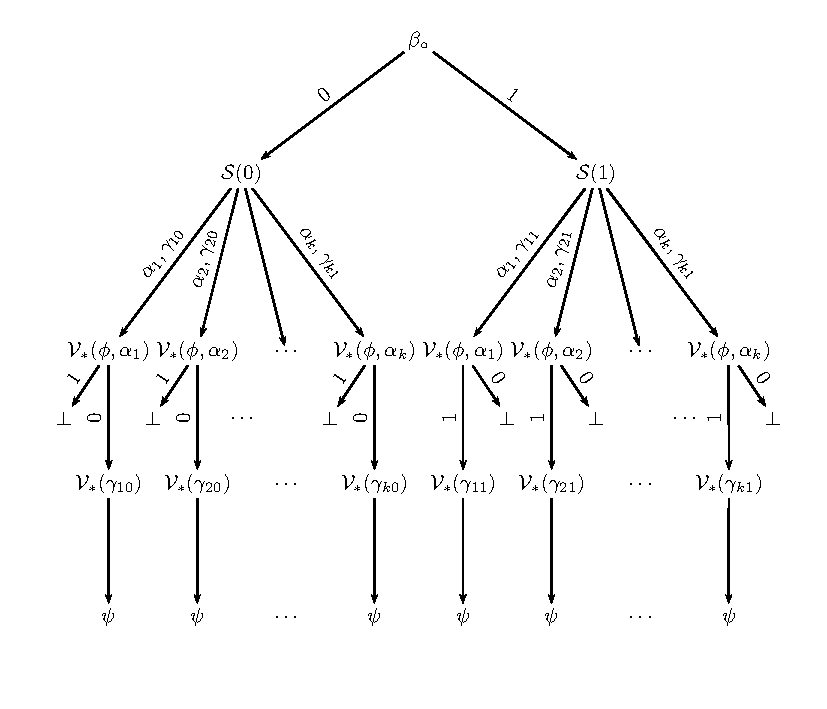
\includegraphics[scale=0.55]{figures/1101-event-tree-ii}
   \caption{Event trees for real protocol execution and for the protocol simulation.}
   \label{fig:event-trees}
\end{figure}

Figure~\ref{fig:event-trees} shows that there are many ways to obtain $\psi$ as an output. During the protocol execution, the prover $\PPP$ chooses uniformly a challenge $\alpha$ by computing $\alpha\gets r^2$ for $r\getsu\ZZ_N^*$. Next, $\VVV_*$ chooses $\beta$ based on its previous knowledge $\phi$ and the commitment $\alpha$. After that the prover $\PPP$ computes the unique reply $\gamma\gets rs^\beta$. The verifier $\VVV_*$ then processes the obtained information and produces an output. With some probability for each path in the event tree the outcome is $\psi$. During the simulation $\beta_\circ$ is chosen uniformly. After that the sub-simulator $\SSS$ creates matching $\alpha,\gamma$ values. Note that the number of possible commitments $\alpha$ that simulator outputs is still $k$. Moreover, the distribution of $\alpha$ values is still uniform for fixed $\beta_\circ$, since the simulator must sample protocol transcripts with the same probability that they occur in the   protocol where both parties are honest. After that the simulator feeds $\phi$ and $\alpha$ value to $\VVV_*$ to obtain $\beta$. If $\beta=\beta_\circ$, the maching response is fed into $\VVV_*$ to obtain the output. If $\beta\neq\beta_\circ$, the simulator halts abruptly.   
 
At first glance, you may get a deceptive feeling that all paths are equally provable in the real protocol run. This is not true because $\VVV_*(\phi,\alpha)$ may bias the output $\beta$ depending on the value of $\alpha$. For the similar reason, the claim that in path during the simulation we reach $\bot$ is $\frac{1}{2}$ is incorrect. However, if we consider path pairs that go through $\alpha_i$ in the simulation, the potential bias cancels out. Thus, we can straightforwardly prove 
\begin{align*}
\pr{
\begin{aligned}
 &\beta_\circ\getsu\set{0,1},\alpha,\gamma\gets\SSS(\beta_\circ),\\
 &\beta\gets\VVV_*(\phi,\alpha):\beta\neq\beta_\circ\wedge\alpha=\alpha_0
\end{aligned}
}=%
\frac{1}{2}\cdot\frac{1}{k}\cdot
\pr{\VVV_*(\phi,\alpha_0)=0}
+
\frac{1}{2}\cdot\frac{1}{k}\cdot
\pr{\VVV_*(\phi,\alpha_0)=1}=\frac{1}{2k}\enspace
\end{align*}
for any $\alpha_0$. Consequently, 
\begin{align*}
\pr{
\begin{aligned}
 &\beta_\circ\getsu\set{0,1},\alpha,\gamma\gets\SSS(\beta_\circ),\\
 &\beta\gets\VVV_*(\phi,\alpha):\beta\neq\beta_\circ
\end{aligned}
}=\sum_{\alpha_0} \pr{
\begin{aligned}
 &\beta_\circ\getsu\set{0,1},\alpha,\gamma\gets\SSS(\beta_\circ),\\
 &\beta\gets\VVV_*(\phi,\alpha):\beta\neq\beta_\circ\wedge\alpha=\alpha_0
\end{aligned}
}
= \frac{1}{2}\enspace.
\end{align*}

As the second step note that there is a direct one-to-one correspondence of event paths in the real protocol execution and event paths without abortion in the simulation. Namely, each path is determined by $\alpha$ and $\beta$ value. Let us now establish how the probabilities of these paths are related:
\begin{align*}
\pr{
\begin{aligned}
 &\beta_\circ\getsu\set{0,1},\alpha,\gamma\gets\SSS(\beta_\circ): \beta_\circ=\beta_0\\
 &\VVV_*(\phi,\alpha)=\beta_0\wedge\alpha=\alpha_0\wedge\gamma=\gamma(\alpha_0,\beta_0)
\end{aligned}
}=%
\frac{1}{2}\cdot
\pr{
\begin{aligned}
&\alpha,\gamma\gets\SSS(\beta_0): \VVV_*(\phi,\alpha_0)=\beta_0\\
&\alpha=\alpha_0 \wedge \gamma=\gamma(\alpha_0,\beta_0)
\end{aligned}}
\end{align*}   
where $\gamma(\alpha_0,\beta_0)$ denotes the correct response for $\alpha_0$ and $\beta_0$.  
As the simulation always yields a correct response $\gamma$ and the first message is uniformly distributed even for fixed $\beta_0$, we get
\begin{align*}
\pr{
\begin{aligned}
 &\beta_\circ\getsu\set{0,1},\alpha,\gamma\gets\SSS(\beta_\circ): \beta_\circ=\beta_0\\
 &\VVV_*(\phi,\alpha)=\beta_0\wedge\alpha=\alpha_0\wedge\gamma=\gamma(\alpha_0,\beta_0)
\end{aligned}
}=\frac{1}{2k}\cdot\pr{\VVV_*(\phi,\alpha_0)=\beta_0}\enspace.
\end{align*}
The potability that we choose the corresponding path in the real protocol execution is 
\begin{align*}
\pr{
\begin{aligned}
 &\alpha\gets\PPP, \beta\gets\VVV_*(\phi,\alpha):\\ 
 &\alpha=\alpha_0\wedge\beta=\beta_0
\end{aligned}
}=\frac{1}{k}\cdot\pr{\VVV_*(\phi,\alpha_0)=\beta_0}\enspace.
\end{align*}
Thus, we have proven that the probability of simulated paths is exactly twice lower than in the real protocol. 

These two facts make the computation of the statistical distance straightforward. Recall that the statistical distance is the maximal advantage of any distinguisher. Also, recall that the bound is achieved by Neyman-Pearson distinguiher, which for each input $x$ outputs the class for which the probability  of getting $x$ is larger. In our case,
\begin{align*}
\AD_{\text{np}}(\psi_0)=
\begin{cases}
0 & \text{if } \psi_0\neq \bot\enspace,\\
1 & \text{if } \psi_0 = \bot\enspace,
\end{cases}
\end{align*} 
since probability of obtaining $\psi\neq\bot$ must be twice as low in the simulation as in the real protocol. As the corresponding advantage 
\begin{align*}
\abs{\pr{\AD_{\text{np}}(\psi_0)=1|\HHH_0}- \pr{\AD_{\text{np}}(\psi_0)=1|\HHH_1}}=\frac{1}{2}\enspace,
\end{align*}
we have proven the claim.

\vspace*{2ex}
\noindent
\textsc{Proof based on game rewriting.}
Another alternative for proving the desired claim is a systematic rewriting of the simulator constructor until we reach the code from which the claim is more or less evident.  First, recall that the zero-knowledge property of sigma protocols is defined through the equivalence of following games:
\begin{align*}
\begin{game}{\BGAME_0^\ADB}
& \alpha\gets\PPP\\
& \beta\gets\set{0,1}\\
& \gamma\gets\PPP(\beta)\\
& \RETURN \ADB(\alpha,\beta,\gamma)
\end{game}
\qquad\qquad
\begin{aligned}
\begin{game}{\BGAME_1^\ADB}
& \beta\getsu\set{0,1}\\
& \alpha,\gamma\gets \SSS(\beta)\\
& \RETURN \ADB(\alpha,\beta,\gamma)\enspace.
\end{game}\\
\ \\
\end{aligned}
\end{align*}
That is, for any distinguishing algorithm $\ADB$ the distinguishing advantage is zero:
\begin{align*}
\ADVIND{\BGAME_0,\BGAME_1}{\ADB}=
\abs{\pr{\BGAME_0^\ADB=1}-\pr{\BGAME_1^\ADB=1}}=0\enspace.
\end{align*}
In other terms, the distributions of $(\alpha,\beta,\gamma)$ generated in both games coincide. As a consequence, we can rewrite the simulator constructor in the following way: 
\begin{align*}
\begin{aligned}
\begin{fblock}{\VVV_\circ(\phi)}
 &\beta_\circ\getsu\set{0,1}\\
 &(\alpha,\gamma)\gets\SSS(\beta_\circ)\\
 &\beta\gets\VVV_*(\phi,\alpha)\\
 &\IF \beta\neq \beta_\circ\ \THEN \RETURN \bot\\
 &\ELSE \RETURN \VVV_*(\gamma) 
\end{fblock}\\
\
\end{aligned}
\REWRITE
\begin{fblock}{\VVV_\circ(\phi)}
 & \alpha\gets\PPP\\
 & \beta_\circ\gets\set{0,1}\\
 & \gamma\gets\PPP(\beta_\circ)\\
 &\beta\gets\VVV_*(\phi,\alpha)\\
 &\IF \beta\neq \beta_\circ\ \THEN \RETURN \bot\\
 &\ELSE \RETURN \VVV_*(\gamma)\enspace. 
\end{fblock}
\end{align*}
Since $\VVV_*$ response $\beta$ depends only on $\alpha$, we can move the statement upwards together with the if block:
\begin{align*}
\begin{fblock}{\VVV_\circ(\phi)}
 & \alpha\gets\PPP\\
 & \beta_\circ\gets\set{0,1}\\
 & \gamma\gets\PPP(\beta_\circ)\\
 &\beta\gets\VVV_*(\phi,\alpha)\\
 &\IF \beta\neq \beta_\circ\ \THEN \RETURN \bot\\
 &\ELSE \RETURN \VVV_*(\gamma) 
\end{fblock}
\REWRITE
\begin{fblock}{\VVV_\circ(\phi)}
 & \alpha\gets\PPP\\
 & \beta\gets\VVV_*(\phi,\alpha)\\
 & \beta_\circ\gets\set{0,1}\\
 & \IF \beta\neq \beta_\circ\ \THEN \RETURN \bot\\
 & \gamma\gets\PPP(\beta)\\
 &\ELSE \RETURN \VVV_*(\gamma)\enspace. 
\end{fblock}
\end{align*}
From this it is clear that the simulator outputs $\bot$ with the probability $\frac{1}{2}$, since $\beta_\circ$ is generated independently after the $\beta$ is fixed. The reasoning is fundamentally the same we obtained by analysing the event trees. The code rewriting steps that do not alter the semantics of the program literally reshape the event trees without altering the output distribution and thus implicitly mimic the analytic reasoning without nasty details. 

As the refactored simulator code outputs $\bot$ with probability $\frac{1}{2}$ we can simplify the code even further:
\begin{align*}
\begin{fblock}{\VVV_\circ(\phi)}
 & \alpha\gets\PPP\\
 & \beta\gets\VVV_*(\phi,\alpha)\\
 & \beta_\circ\gets\set{0,1}\\
 & \IF \beta\neq \beta_\circ\ \THEN \RETURN \bot\\
 & \gamma\gets\PPP(\beta)\\
 &\ELSE \RETURN \VVV_*(\gamma)\enspace. 
\end{fblock}
\REWRITE
\begin{fblock}{\VVV_\circ(\phi)}
 & \alpha\gets\PPP\\
 & \beta\gets\VVV_*(\phi,\alpha)\\
 & b\getsu\set{0,1}\\
 & \IF b= 0\ \THEN \RETURN \bot\\
 & \gamma\gets\PPP(\beta)\\
 &\ELSE \RETURN \VVV_*(\gamma)\enspace. 
\end{fblock}
\REWRITE
\begin{fblock}{\VVV_\circ(\phi)}
 & b\getsu\set{0,1}\\
 & \IF b= 0\ \THEN \RETURN \bot\\
 & \alpha\gets\PPP\\
 & \beta\gets\VVV_*(\phi,\alpha)\\
 & \gamma\gets\PPP(\beta)\\
 &\ELSE \RETURN \VVV_*(\gamma)\enspace. 
\end{fblock}
\end{align*}
From this representation it is also evident that 
\begin{align*}
\pr{\VVV_\circ(\phi)=\psi}=\frac{1}{2}\cdot
\pr{\alpha\gets\PPP, \beta\gets\VVV_*(\phi,\alpha),\gamma\gets\PPP(\alpha):\VVV_*(\gamma)=\phi} \enspace.
\end{align*}
After that the reasoning about the statistical distance is identical to the approach used in the first proof.

\end{solution}
\end{document}

